
\chapter[Desenvolvimento]{Desenvolvimento}

O Desenvolvimento (segunda parte do Corpo do Trabalho) é subdividido em seções de acordo com o planejamento do autor. É exigido organização, objetividade e clareza. É conveniente dividi-lo nas seguintes partes:

\begin{itemize}

	\item Projeto, requisitos e outras definições sobre o problema a ser resolvido, identificado em seções anteriores.
	\item Implementação do projeto, discussões sobre codificação (se aplicado ao tema).
	\item Avaliação, testes ou outras análises sobre o projeto, direcionando o leitor para as conclusões do projeto.

\end{itemize}



\section{Corpo do Texto}

O estilo de redação deve atentar a boa prática da linguagem técnica. Para a terminologia metrological usar o Vocabulário Internacional de Termos Fundamentais e Gerais de Metrologia \cite{inmetro2003}  (Instituto Nacional de Metrologia, 2003).

Grandezas dimensionais devem ser apresentadas em unidades consistentes com  o Sistema Internacional de Unidades  (SI). Outras unidades podem ser usadas  como unidades secundárias entre parenteses se necessário. Exceções são relacionadas a unidades não-SI usadas como identificadores comerciais como pro exemplo \lq\lq disquete de  3$\nicefrac{1}{2}$ polegadas\rq\rq. 

Na apresentação de números ao longo do texto usar virgula para separar a parte decimal de um número. Resultados experimentais devem ser apresentados com sua respectiva incerteza de medição.

\section{Títulos de capítulos e seções}

Recomendações de formatação de seções. 

\begin{description}

	\item 1 SEÇÃO PRIMÁRIA - MAIÚSCULAS; normal; tamanho 16;

	\item 1.1 Seção Secundária - Minúsculas, com exceção da primeira letra; normal; tamanho 14;

	\item 1.1.1 Seção terciária - Minúsculas, com exceção da 
	primeira letra; normal; tamanho 12;

	\item Os demais níveis seguem formatação do nível acima. 

\end{description}



\section{Notas de rodapé}

Notas eventualmente necessárias devem ser numeradas de forma sequencial ao longo do texto no formato 1, 2, 3... sendo posicionadas no rodapé de cada página na qual a nota é utilizada.\footnote{Como, por exemplo, esta nota}.

\section{Legendas}

As legendas devem ser numeradas sequencialmente e agrupadas sobre um conjunto. Os grupos de legendas são, por exemplo, os de Figuras, Equações, Quadros, Tabelas e Algoritmos. O número sequencial pode fazer relação com a seção mas isto não é obrigatório. As seções a seguir descrevem detalhes sobre estes conjuntos.

\section{Equações}

Equações matemáticas devem ser numeradas sequencialmente e alinhadas a esquerda com recuo de 0,6 cm. Usar numerais arábicos entre parênteses, alinhado a direita, no formato Times New Roman de 9 pts. para numerara as equações como mostrado na Eq. (\ref{eqn01}).

Referências a equações no corpo do texto devem ser feitas como \lq\lq Eq. (\ref{eqn01})\rq\rq\ quando no meio de uma frase ou como \lq\lq Equação (\ref{eqn01})\rq\rq\ quando no inicio de uma sentença. Um espaçamento de 11 pontos deve ser deixado acima, abaixo e entre equações subsequentes. Para uma apresentação compacta das equações deve-se usar os símbolos e expressões matemáticas mais adequados e parênteses para evitar ambiguidades em denominadores. Os símbolos usados nas equações citados no texto devem apresentar exatamente a mesma formatação usada nas equações.
\begin{equation}
\label{eqn01}
	\frac{d\mathbf{C}}{dw} = \frac{du}{dw}\cdot \mathbf{F}_u + 
		\frac{dv}{dw}\cdot \mathbf{F}_v 
\end{equation}

O significado de todos os símbolos mostrados nas equações deve ser apresentado na lista de símbolos no inicio do trabalho, embora, em certas circunstancias o autor possa para maior clareza descrever o significado de certos símbolos no corpo do texto, logo após a equação.


\section{Figuras e Gráficos}

As figuras devem ser centradas entre margens e identificadas por uma legenda alinhada a esquerda com recuo especial de deslocamento de 1,8 cm, com mostrado 
na Fig. (\ref{fig01}). O tamanho das fontes empregadas nos rótulos e anotações 
usadas nas figuras deve ser compatível com o usado no corpo do texto. Rótulos e 
anotações devem estar em português, com todas as grandezas mostradas em 
unidades do SI (Sistema Internacional de unidades).

Todas as figuras, gráficos e fotografias devem ser numeradas e referidas no 
corpo do texto adotando uma numeração sequencial de identificação. As figuras e 
gráficos devem ser claras e com qualidade adequada para eventual reprodução 
posterior tanto em cores quanto em preto-e-branco.


As abscissas e ordenadas de todos os gráficos devem ser rotuladas com seus 
respectivos títulos em português seguida da unidade no SI que caracteriza a 
grandes entre colchetes. 

\begin{figure}[hbt!]
	\centering
		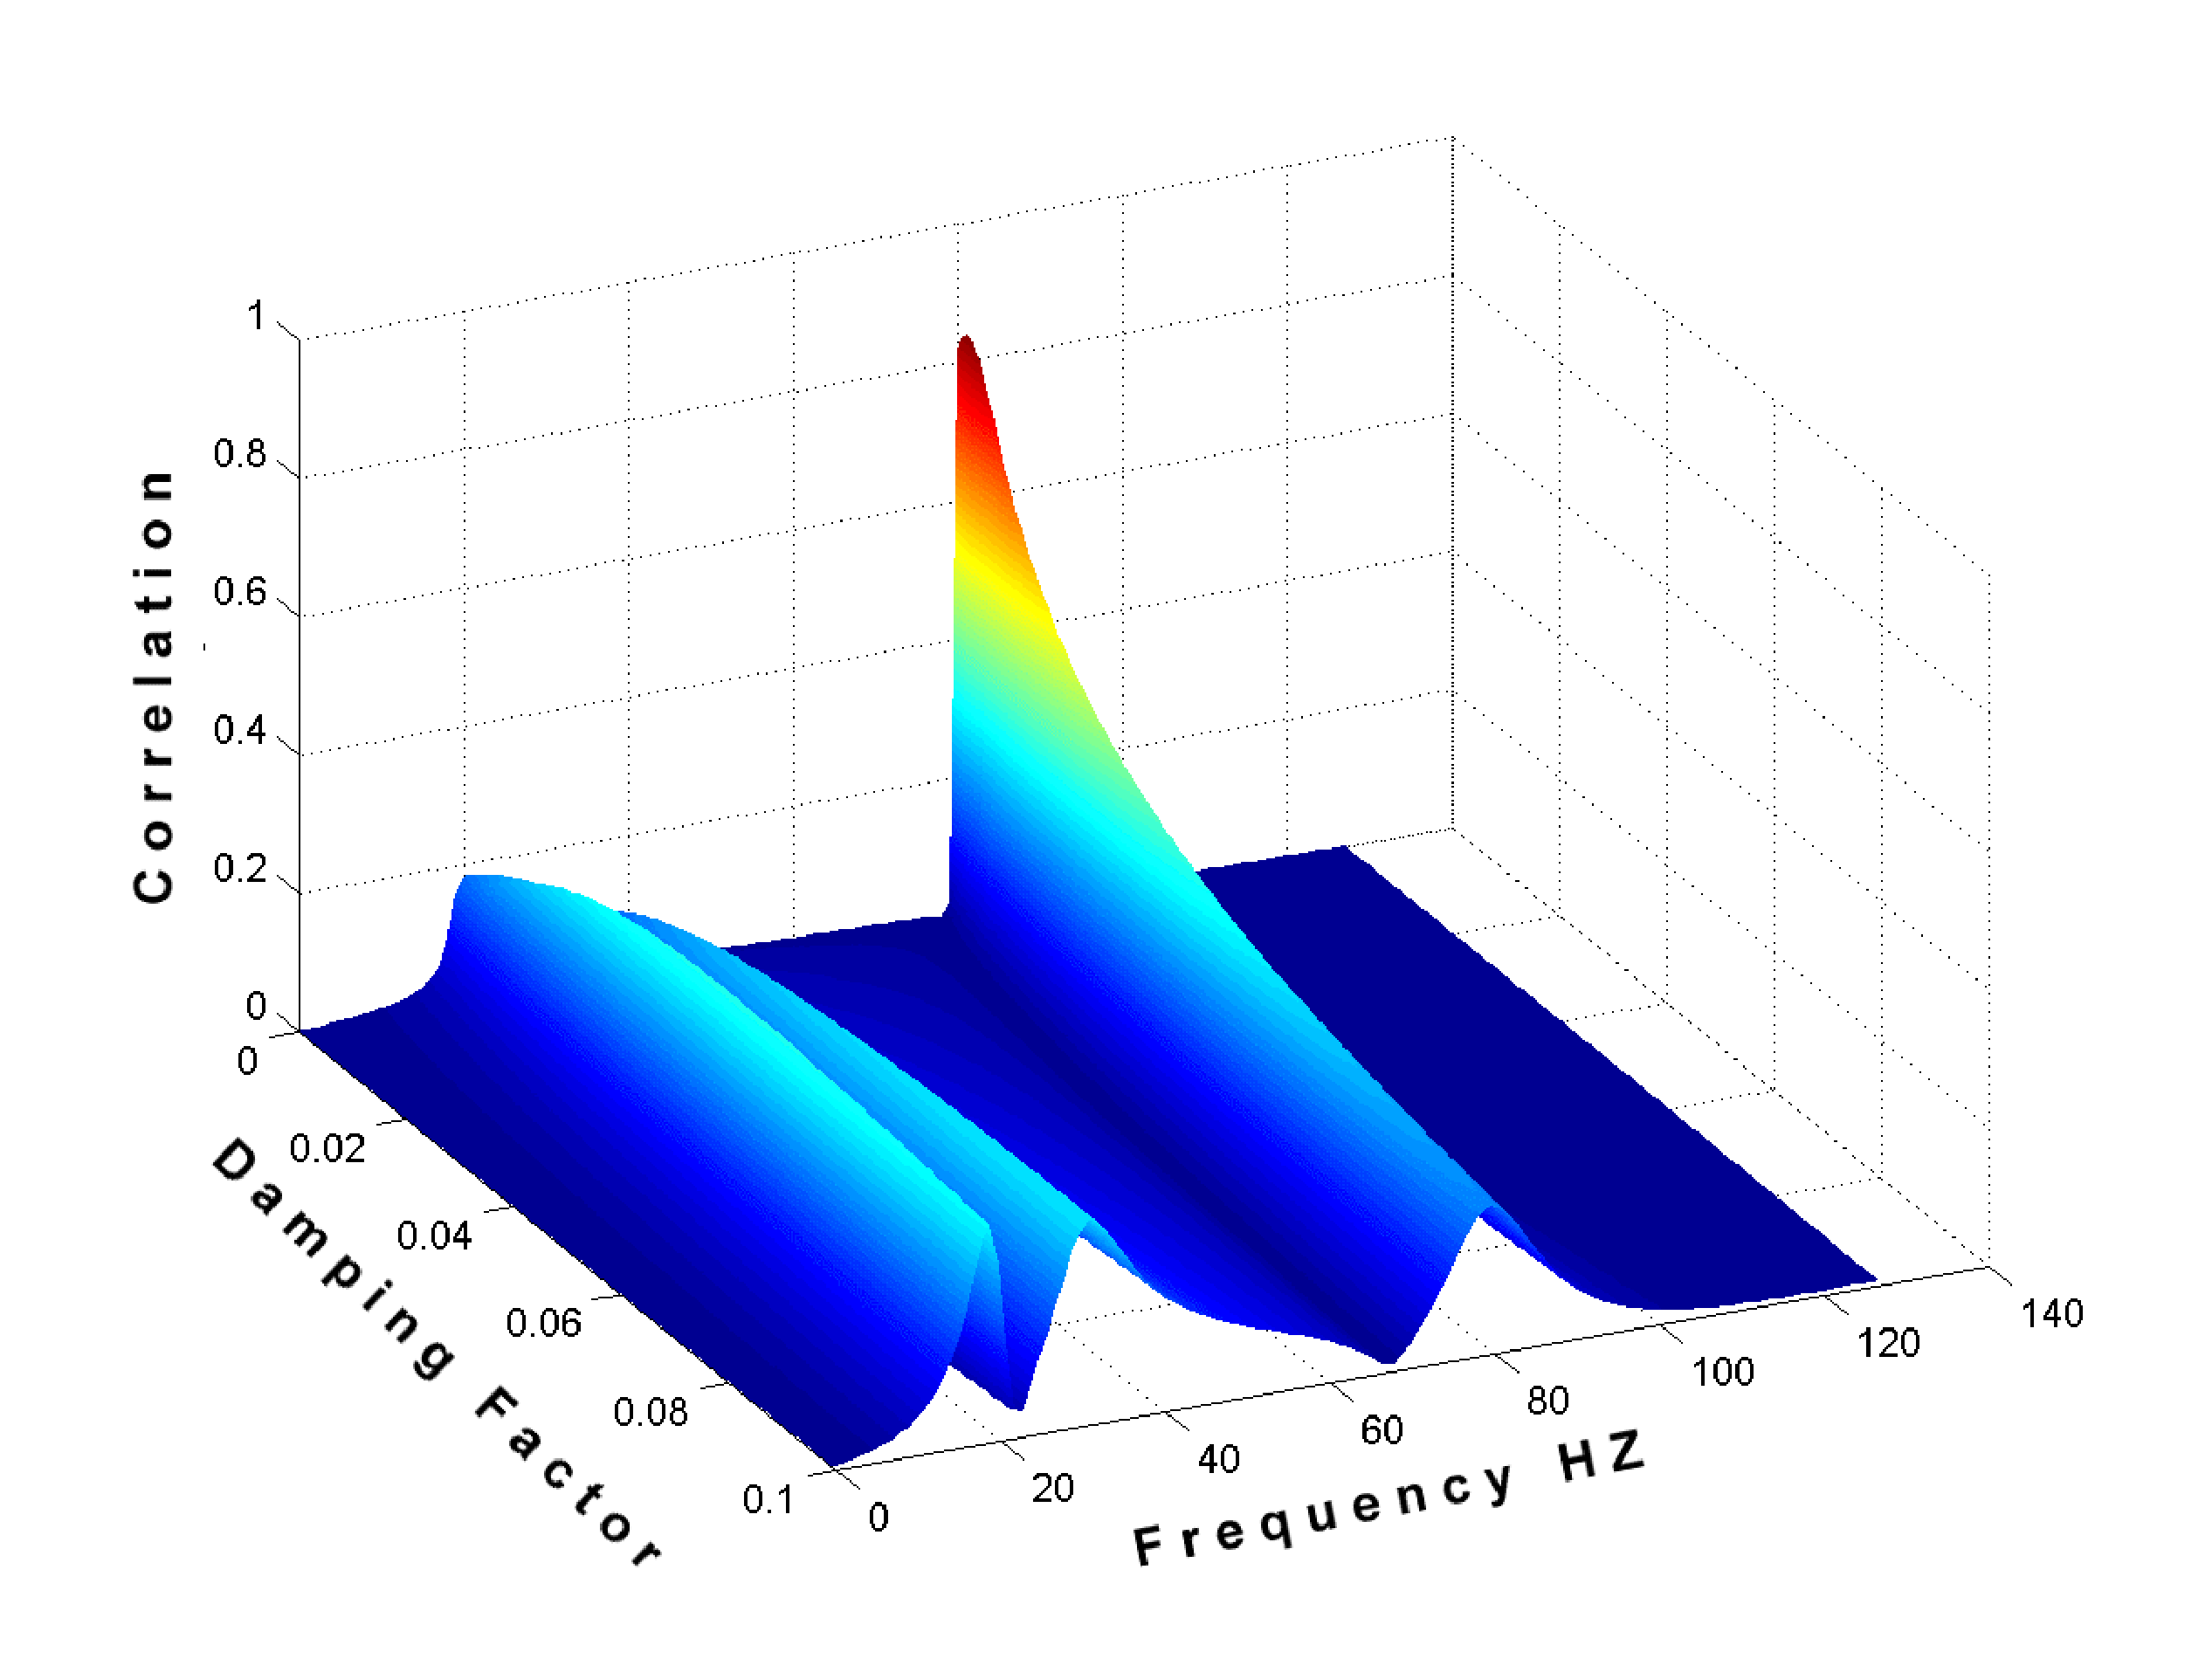
\includegraphics[keepaspectratio=true,scale=0.3]{imagens/fig01.eps}
	\caption{Correlação de coeficientes Wavelets.}
	\label{fig01}
\end{figure}


A referência explícita no texto à uma figura deve ser feita como 
\lq\lq Fig. (\ref{fig01})\rq\rq\ quando no meio de uma frase ou como 
\lq\lq Figura (\ref{fig01})\rq\rq\ quando no início da mesma. Referencias 
implícitas a uma dada figura devem ser feitas entre parênteses como 
(Fig. \ref{fig01}). Para referências a mais de uma figura as mesmas regras 
devem ser aplicadas usando-se o plural adequadamente. Exemplos:

\begin{itemize}
	\item \lq\lq Após os ensaios experimentais, foram obtidos os resultados 
	mostrados na Fig. (\ref{fig01}), que ...\rq\rq
	\item \lq\lq A Figura (\ref{fig01}) apresenta os resultados obtidos, onde 
	pode-se observar que ...\rq\rq
	\item \lq\lq As Figuras (1) a (3) apresentam os resultados obtidos, 
	...\rq\rq
	\item \lq\lq Verificou-se uma forte dependência entre as variáveis citadas 
	(Fig. \ref{fig01}), comprovando ...\rq\rq
\end{itemize}

É recomendado (não obrigatório) que cada figura deve ser posicionada o mais próxima possível da primeira citação feita à mesma no texto, imediatamente após o parágrafo no qual é feita tal citação, se possível, na mesma página.


\section{Tabela}

As tabelas devem estar centradas entre margens e identificadas por uma legenda alinhada a esquerda, com recuo especial de deslocamento de 1,8 cm, posicionada acima da tabela com mostrado nas Tabs. (\ref{tab01}) e (2), a título de exemplo. O tamanho das fontes empregadas nos rótulos e anotações usadas nas 
tabelas deve ser compatível com o usado no corpo do texto. Rótulos e anotações devem estar em português. Um espaçamento de 11 pts deve ser deixado entre a legenda e a tabela, bem como após a tabela.

As grandezas dimensionais mostradas em cada tabela devem apresentar unidades consistentes com o SI. As unidades de cada variável devem ser mostradas apenas na primeira linha e/ou coluna da tabela, entre colchetes.

\begin{table}[hbt!]
	\centering
% 	\resizebox{\textwidth}{!}{\begin{tabular}{ccc}
	\begin{tabular}{ccc}
		\toprule
		\textbf{Processing type} & \textbf{Property 1} (\%) & 
		\textbf{Property 2} $[\mu m]$ \\
		\midrule
		Process 1 & 40.0 & 22.7 \\
		Process 2 & 48.4 & 13.9 \\
		Process 3 & 39.0 & 22.5 \\
		Process 4 & 45.3 & 28.5 \\
		\bottomrule
	\end{tabular}
% 	\end{tabular}}
	\caption{Propriedades obtidas após processamento}
	\label{tab01}
\end{table}

A referência explícita no texto à uma dada tabela deve ser feita como \lq\lq Tab. (\ref{tab01})\rq\rq\ quando no meio de uma frase ou como \lq\lq Tabela (\ref{tab01})\rq\rq\ quando no início da mesma. Referências implícitas a uma dada tabela devem ser feitas entre parênteses como \lq\lq (Tab. \ref{tab01}). Para referências a mais de uma tabela as mesmas regras devem ser aplicadas usando-se o plural adequadamente. Exemplos:

\begin{itemize}
	\item \lq\lq Após os ensaios experimentais, foram obtidos os resultados 
	mostrados na Tab. (\ref{tab01}), que ...\rq\rq
	\item \lq\lq A Tabela (\ref{tab01}) apresenta os resultados obtidos, onde 
	pode-se observar que ...\rq\rq
	\item As Tabelas (1) a (X) apresentam os resultados obtidos, ...\rq\rq
	\item Verificou-se uma forte dependência entre as variáveis citadas 
	(Tab. \ref{tab01}), comprovando ...\rq\rq
\end{itemize}

Cada tabela deve ser posicionada o mais próxima possível da primeira citação 
feita à mesma no texto, imediatamente após o parágrafo no qual é feita a 
citação, se possível, na mesma página.


\section{Códigos-fonte}

Para a listagem de código-fonte recomenda-se a formatação conforme o algoritmo~\ref{code:py}, veja configuração \textit{lstset} em fixos/setup.tex. A configuração é fonte Teletypefont ou Courier, mono-espaçada, de tamanho 10pt, com numeração de linhas (cores da sintaxe da linguagem de programação não obrigatórias). A numeração de linhas não é obrigatória mas é recomendável para melhor explicação durante o desenvolvimento do trabalho. Figuras (\textit{screenshots}) de códigos-fonte podem ser utilizados como alternativa (é necessário ter cuidado com a visualização do código na imagem como foco e tamanho das letras).
\\

\begin{lstlisting}[language=Python, caption=Exemplo em Python, captionpos=b, label=code:py]
import numpy as np
 
def incmatrix(genl1,genl2):
    m = len(genl1)
    n = len(genl2)
    M = None #to become the incidence matrix
    VT = np.zeros((n*m,1), int)  #dummy variable
 
    #compute the bitwise xor matrix
    M1 = bitxormatrix(genl1)
    M2 = np.triu(bitxormatrix(genl2),1) 
 
    for i in range(m-1):
        for j in range(i+1, m):
            [r,c] = np.where(M2 == M1[i,j])
            for k in range(len(r)):
                VT[(i)*n + r[k]] = 1;
                VT[(i)*n + c[k]] = 1;
                VT[(j)*n + r[k]] = 1;
                VT[(j)*n + c[k]] = 1;
 
                if M is None:
                    M = np.copy(VT)
                else:
                    M = np.concatenate((M, VT), 1)
 
                VT = np.zeros((n*m,1), int)
 
    return M
\end{lstlisting}

\section{Citação de Referências}

Referências a outros trabalhos tais como artigos, teses, relatórios, etc. devem ser feitas no corpo do texto devem estar de acordo com a norma corrente ABNT NBR 6023:2002 (ABNT, 2000), esta ultima baseada nas normas ISO 690:1987:
\begin{itemize}
	\item \lq\lq \cite{bordalo1989}, mostraram que...\rq\rq

	\item \lq\lq Resultados disponíveis em \cite{coimbra1978}, \cite{clark1986} 
	e \cite{sparrow1980}, mostram que...\rq\rq
\end{itemize}

Para referências a trabalhos com até dois autores, deve-se citar o nome de ambos os autores, por exemplo: \lq\lq \cite{soviero1997}, mostraram que...\rq\rq

Ainda podem ser utilizados outras formas de citações tal como "Segundo \citeauthoronline{coimbra1978} (\citeyear{coimbra1978}), é definido que a...".

